\subsection{Ablation studies}

\subsubsection{Fine tuning \llamavtwo vs. training from scratch on code}\label{sec:scratch}

\begin{figure}[t!]
%\begin{wrapfigure}{R!}{0.35\linewidth}
\centering
\begin{subfigure}[T]{0.32\linewidth}
    \centering
    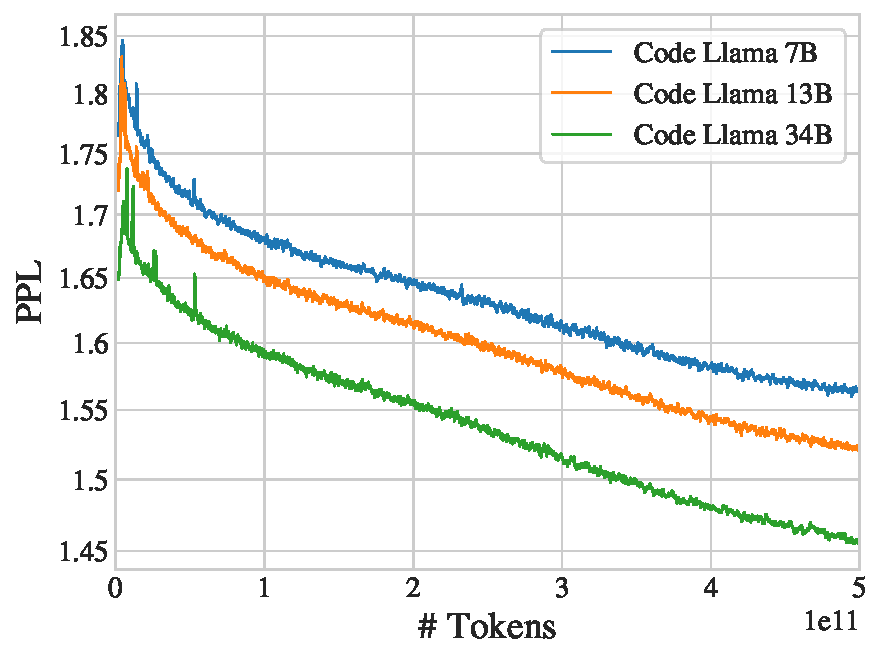
\includegraphics[width=\linewidth]{figs/training_curves_codellama.pdf} % 
    \caption{
    % \textbf{Training losses} of both \model 7B versus an identical model trained from scratch.
    \label{fig:training_curves}}
    %\vspace{-3.5em}
\end{subfigure}
\hfill
\begin{subfigure}[T]{0.32\linewidth}
    \centering
    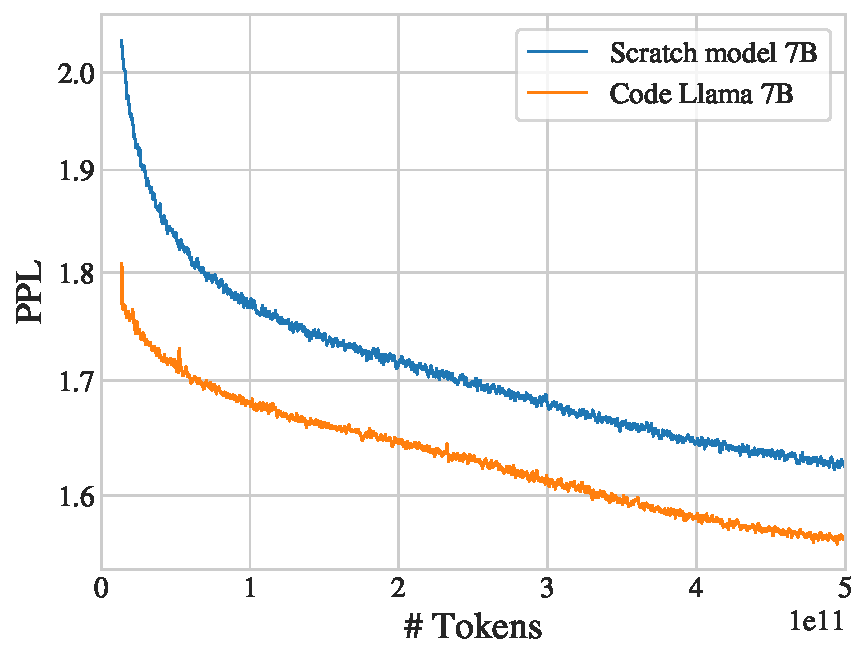
\includegraphics[width=\linewidth]{figs/training_curves_codellama_scratch.pdf} % 
    \caption{
    \label{fig:curves_scratch_ablation_loss}}
\end{subfigure}
\hfill
\begin{subfigure}[T]{0.32\linewidth}
    \centering
    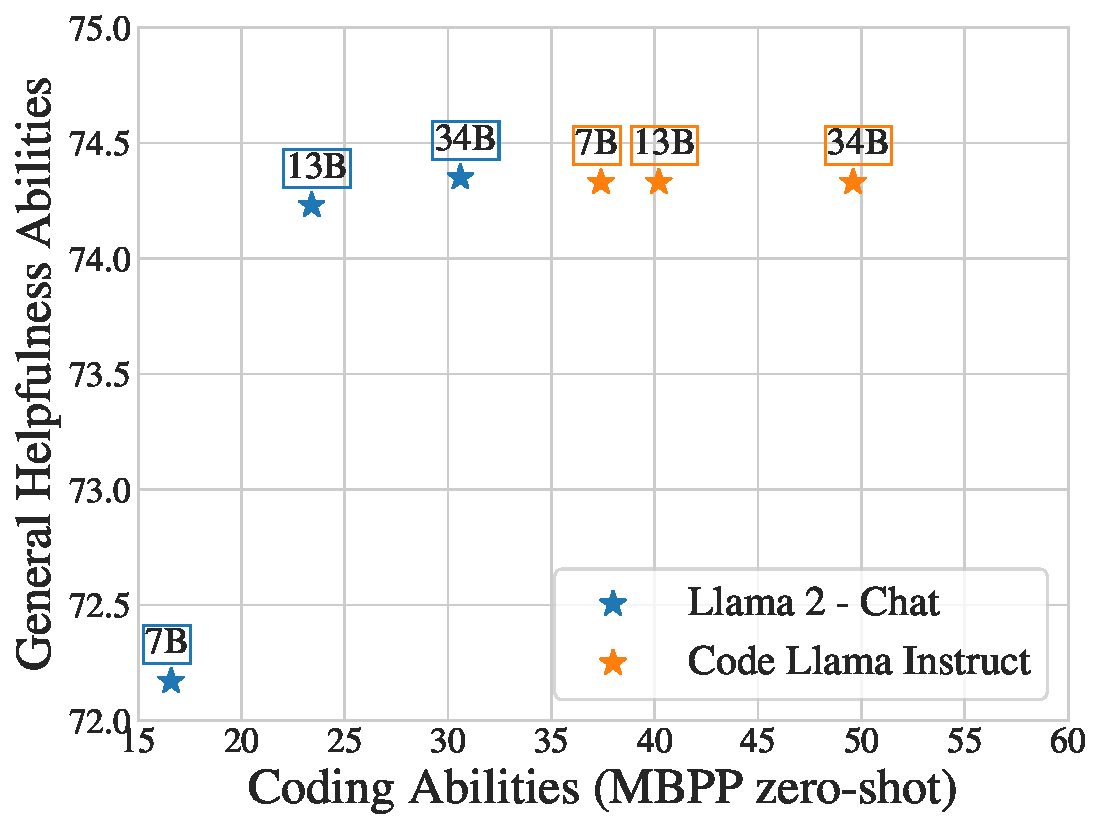
\includegraphics[width=\linewidth]{figs/fig_code_helpful.pdf}
    \caption{
    \label{fig:helpfulness_vs_mbpp}}
\end{subfigure}
\caption{(a) \textbf{Training perplexity of \model models.} The continued decrease at 500B tokens suggests further training would be beneficial. Results are presented without infilling for 7B and 13B models. (b) \textbf{Training losses} of both \model 7B versus an identical model trained from scratch (c) \textbf{MBPP (coding benchmark) vs. Helpfulness} according to the helpfulness reward model from \llamavtwo~\citep{touvron2023llamav2}.}
\end{figure}


\model is based on the \llamavtwo models, which are trained on 2T tokens of text, including only 80B tokens of code. 
We tune these models on 500B extra tokens, consisting mostly of code (85\%). 
Figure~\ref{fig:training_curves} shows the training curves of \model. 


We compare the 7B parameters model to an identical model trained from scratch on the same data mix (Figure~\ref{fig:curves_scratch_ablation_loss}). At the end of training, the loss of the model trained from scratch is equal to the loss of \model 7B at about half of its training (with 240B less training tokens). Moreover, this gap becomes larger over time. 


\subsubsection{Instruction fine-tuning}\label{sec:inst_results}
\paragraph{General helpfulness vs. coding ability}

We evaluate \instmodel and compare it to \llamavtwo-Chat for coding tasks and helpfulness (\Cref{fig:helpfulness_vs_mbpp}). 
We observe that \model improves its coding abilities for each model sizes, while preserving the general helpfulness performance inherited from \llamavtwo. 
The results on the helpfulness axis is an indication that \model performs greatly on general instructions following. 
But we emphasize that this result should be taken with a grain of salt, since we limited our automatic evaluation to scoring the models answers with \llamavtwo reward model.

\paragraph{The value of self-instruct data}

We also perform ablations, showing the value of the self-instruct data that we generate with our own model. 
To evaluate the capacity of the model to answer questions, we use a zero-shot version of MBPP. We prompt the model to generate the code between \texttt{[PYTHON]} and \texttt{[/PYTHON]} tags to make it easy to parse the result. Our exact prompt is shown in Figure~\ref{fig:mbpp_zero_prompt} in the Appendix.
Table~\ref{tab:self_instruct} show the impact of training on data generated using our models and filtered with unit tests as described in Section~\ref{sec:instruct}. The self-instruct data allows us to improve our scores on benchmarks such as HumanEval and MBPP. It also makes the training more reliable. With self-instruct, the model easily learns to follow the format requested for MBPP zero-shot while it sometimes fails without it.

\begin{table}[t!]
  \center
   \setlength{\tabcolsep}{3pt}
  \begin{tabular}{rcrrr}
  \toprule
  Size&SI&HumanEval& \multicolumn{2}{c}{MBPP} \\
  &&& 3-shot & zero-shot \\
  \midrule
\multirow{ 2}{*}{7B} &\ding{55} &  \acc{30.5}& \acc{43.4} &\acc{37.6}\\
& \ding{51}& \acc{34.8}& \acc{44.4} &\acc{37.4}\\
\midrule
\multirow{ 2}{*}{13B}& \ding{55} & \acc{40.85365} & \acc{46.2}&\acc{20.4}\\
& \ding{51}& \acc{42.7} & \acc{49.4}&\acc{40.2}\\
  \bottomrule
    \end{tabular}
    \caption{\textbf{Impact of self-instruct data.} Impact of self-instruct data (SI) on the MBPP and HumanEval scores of our self-instruct models. The scores are computed using greedy decoding. In MBPP zero-shot, we prompt the model to generate the solution between \texttt{[PYTHON][/PYTHON]} tags. Removing SI results in generally lower scores on HumanEval and MBPP, and makes learning to generate code with the right format for MBPP zero shot much less reliable.}
    \label{tab:self_instruct}
\end{table}

\paragraph{Unnatural model.} For comparison purposes, we also finetuned \pymodel 34B on 15,000 unnatural instructions similarly to~\citet{honovich2022unnatural} using the same prompts as for the self-instruct dataset. We do not release this model, but we observe clear improvements on HumanEval and MBPP which are indicative of the improvements that can be reached with a small set of high-quality coding data. The results of the unnatural model are shown in Table~\ref{tab:main_res}. 



\subsubsection{Pass@k evaluation} We study the effect of the sampling temperature on the pass@k performance. Specifically, we report pass@1, 10, and 100 using temperature $\in \{0.1, 0.4, 0.6, 0.8\}$ on both HumanEval and MBPP. Results are depicted in Figure~\ref{fig:abb_temp}. As expected, as we increase the temperature, the pass@1 scores are getting worse while the pass@10 and pass@100 improve. 

\begin{figure}[t!]
     \centering
     \begin{subfigure}[b]{0.32\textwidth}
         \centering
         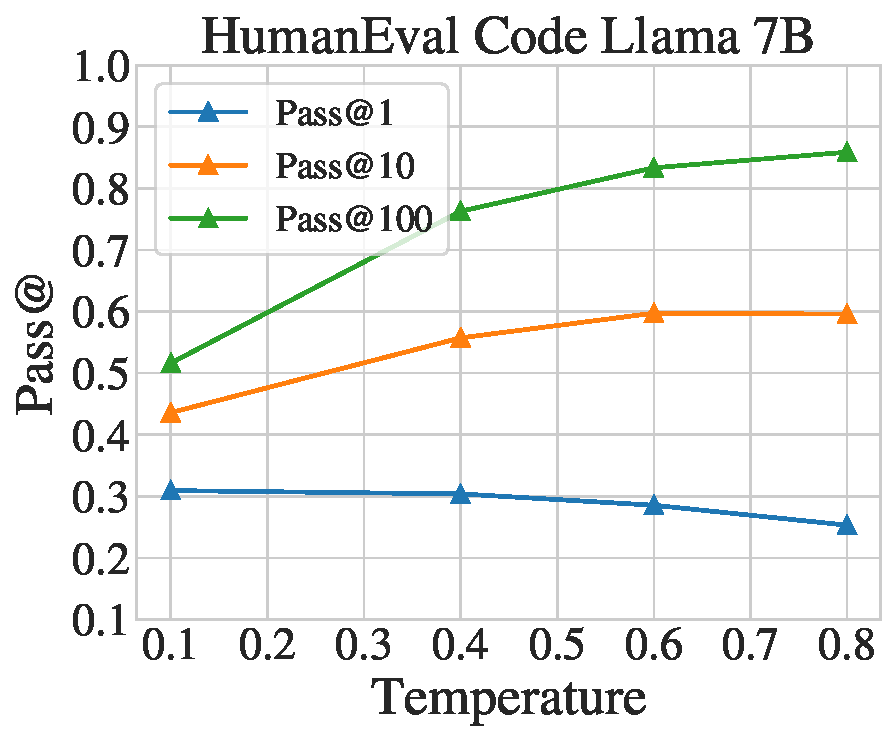
\includegraphics[width=\textwidth]{figs/human_eval_CodeLLaMA_7B.pdf}         
     \end{subfigure}
     \hfill
     \begin{subfigure}[b]{0.32\textwidth}
         \centering
         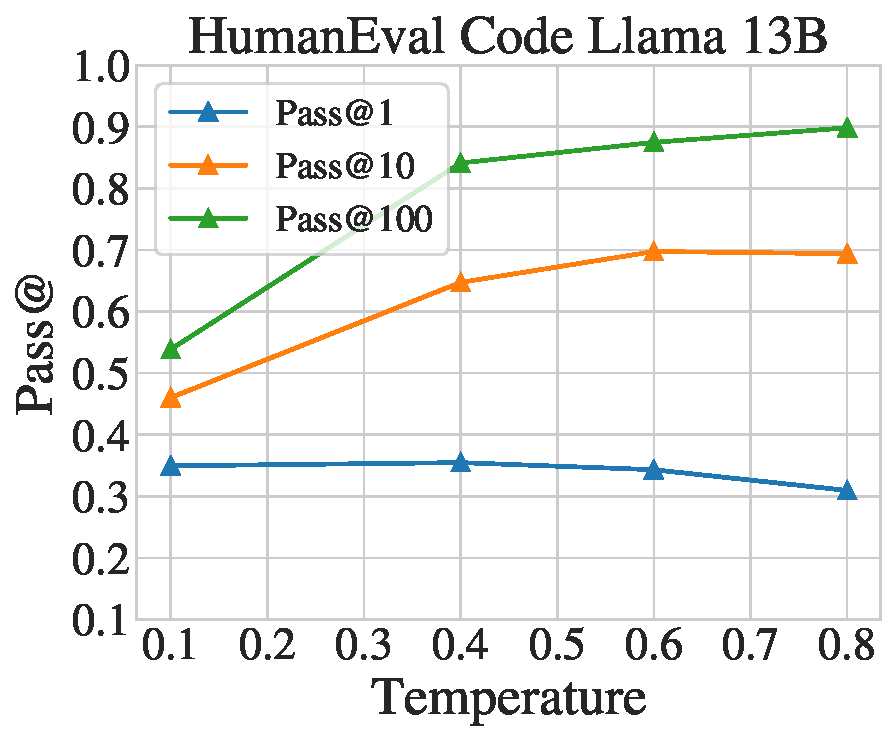
\includegraphics[width=\textwidth]{figs/human_eval_CodeLLaMA_13B.pdf}
     \end{subfigure}
     \hfill
     \begin{subfigure}[b]{0.32\textwidth}
         \centering
         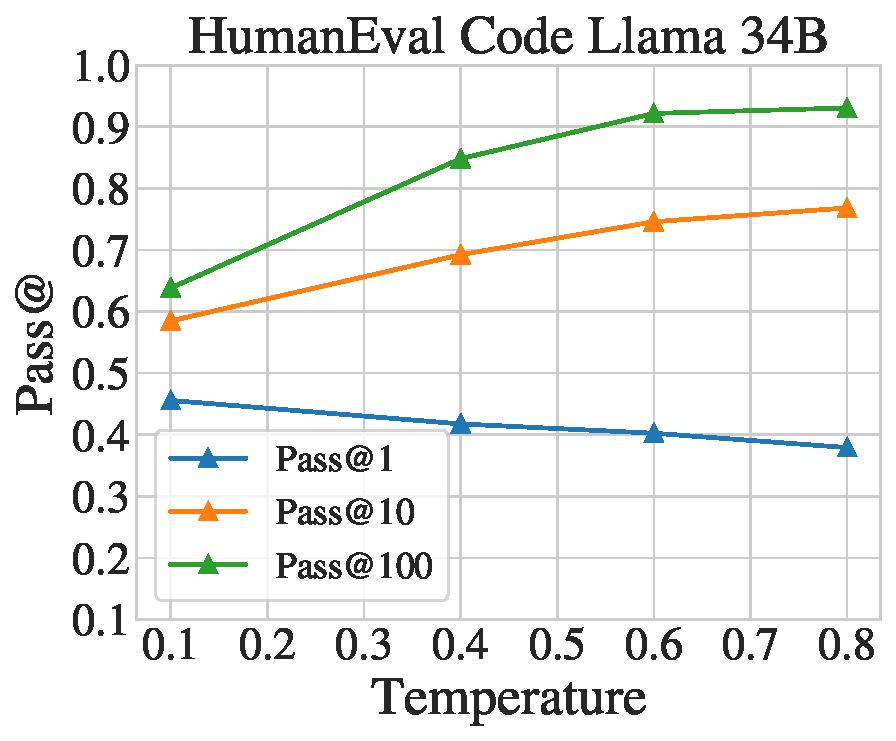
\includegraphics[width=\textwidth]{figs/human_eval_CodeLLaMA_34B.pdf}
     \end{subfigure} \\
     \begin{subfigure}[b]{0.32\textwidth}
         \centering
         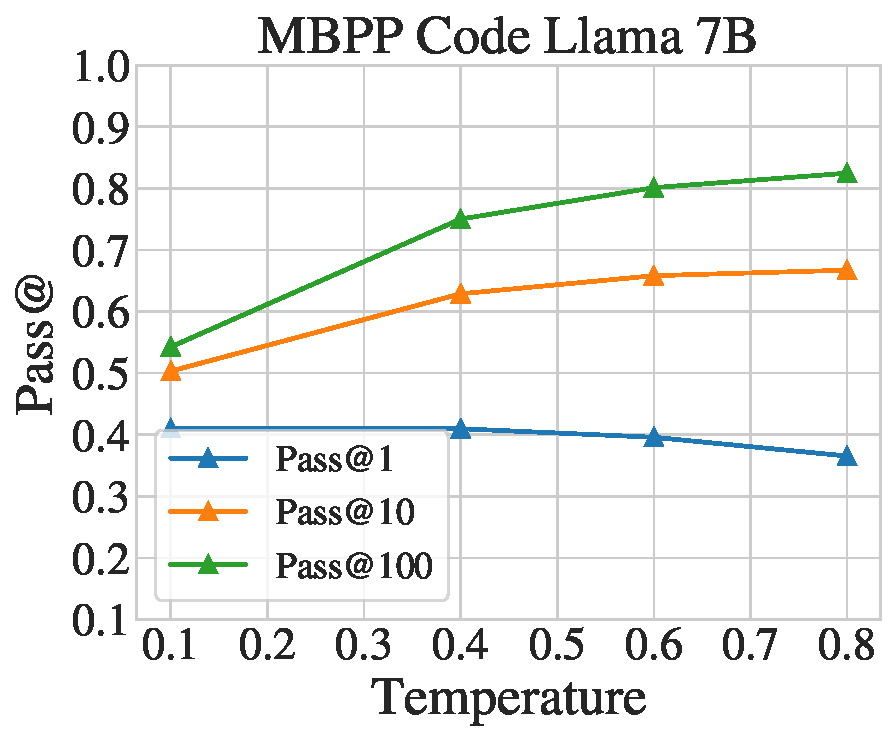
\includegraphics[width=\textwidth]{figs/mbpp_CodeLLaMA_7B.pdf}
     \end{subfigure}
     \hfill
     \begin{subfigure}[b]{0.32\textwidth}
         \centering
         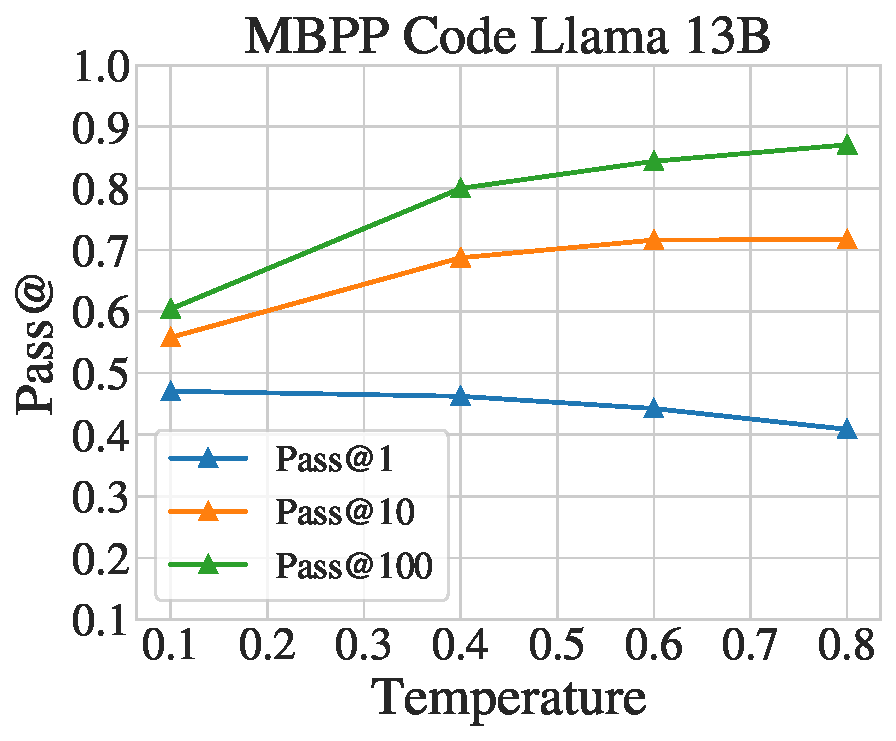
\includegraphics[width=\textwidth]{figs/mbpp_CodeLLaMA_13B.pdf}
     \end{subfigure}
     \hfill
     \begin{subfigure}[b]{0.32\textwidth}
         \centering
         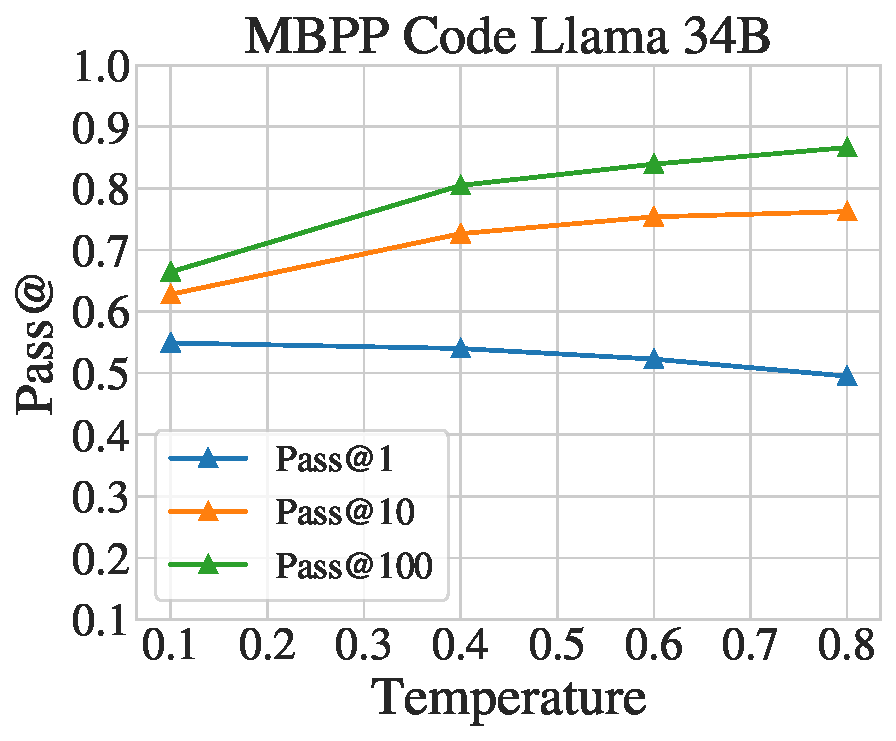
\includegraphics[width=\textwidth]{figs/mbpp_CodeLLaMA_34B.pdf}
     \end{subfigure} \\
    \caption{\textbf{\model scores different temperature values.} Results are presented for 7B, 13B, and 34B models on HumanEval and MBPP benchmarks. We report Pass@1, Pass@10, and Pass@100 for different temperature values. We use nucleus sampling with p=0.95.}
    \label{fig:abb_temp}
\end{figure}
